% ---------------------------------------------------------------------
% HEADER
% Formålet med å legge header til et eget dokument er å garantere at
% oppsettet av dokumentene er likt for alle løsningsforslagene.
% I headeren skjer følgende:
% (1) Dokumentet blir startet
% (2) Pakker blir importert
% ---------------------------------------------------------------------
% ---------------------------------------------------------------------
% HEADER
% Formålet med header er å importere de samme pakkene i alle dokumentene.
% ---------------------------------------------------------------------

% Sett opp dokumentet. Her kan 'twoside' brukes for printing
\documentclass[12pt, a4paper]{article}

% Vi trenger utf-8 for å bruke norske bokstaver: Æ, Ø, Å
\usepackage[utf8]{inputenc}

% Vi setter babel til norsk, da får dokumentegenskaper norske titler
\usepackage[norsk]{babel}

% For å kunne bruke grafikk
\usepackage{graphicx}
\newcommand{\figwidth}{0.75}

% Matematikkpakker fra AMS - American Mathematical Society
\usepackage{amsmath, amsthm, amsfonts, amssymb, mathtools}

% For eventuelle linker, e.g. \href{URL}{text}
\usepackage{hyperref}

% For headers og footers med eventuell logo
\usepackage{fancyhdr}

% Sett marginer manuelt
\usepackage[top = 3cm, left = 3cm, right = 3cm, bottom = 3cm]{geometry}

% For enkle lister, nyttig for oppgave a), b), c), ...
\usepackage[sharp]{easylist}

% Dersom flere kolonner er ønskelig i deler av dokumentet
\usepackage{multicol}

% For luft mellom paragrafer
\usepackage{parskip}

% For logikk assosiert med logoer
\usepackage{ifthen}

% For å finne totalt antall sider
\usepackage{lastpage}

% Annet
\usepackage{enumitem}

\usepackage{polynom}% Polynomer
\polyset{style=C, div=:}

\usepackage{systeme}% Likningssystemer

% Kan brukes når noe stryker ut noe, f.eks 1/n * n, her kan man ta \frac{1}{\cancel{n}} * \cancel{n}
\usepackage{cancel}



% ---------------------------------------------------------------------
% DOKUMENTVARIABLER
% ---------------------------------------------------------------------
\newcommand{\fagkode}{R1}
\newcommand{\semesteraar}{høsten 2017}
\newcommand{\forfatter}{Anita G.}
\newcommand{\dokumenttittel}{Løsningsforslag -- Eksamen \fagkode, \semesteraar}

\usepackage{siunitx}


% Set til 'true' og oppgi logo dersom du vil bruke en logo
\newboolean{bruklogo}
\setboolean{bruklogo}{false}
\newcommand{\logonavn}{}



% ---------------------------------------------------------------------
% SETUP
% Formålet med å legge setup til et eget dokument å garantere at headers,
% footers, og øverste del av dokumentet er likt for alle
% løsningsforslagene.
% ---------------------------------------------------------------------
% ---------------------------------------------------------------------
% HEADER
% Formålet med setup er at dokumentene ser rimelig like ut.
% ---------------------------------------------------------------------


% ---------------------------------------------------------------------
% Alternativ font. Kommentert ut fordi Computer Modern (default) er pen
%\usepackage{kmath,kerkis}
%\usepackage[T1]{fontenc}
% ---------------------------------------------------------------------


% ---------------------------------------------------------------------
% Sett opp headers og footers
\ifthenelse{\boolean{bruklogo}}{
% Dersom logo skal brukes, sett logoen oppe til høyre med bredde 4 cm
	\rhead{\includegraphics[width=3.5cm]{\logonavn}}
}{
% Dersom logo ikke skal brukes, sett tom header
	\rhead{}
} 
\rfoot{\thepage}
\cfoot{}
\lhead{}
\lfoot{{\scriptsize Forbedringsforslag? Bidra på \url{https://github.com/tommyod/matte_eksamener_VGS}.}}
\renewcommand{\headrulewidth}{0pt}
% ---------------------------------------------------------------------


% ---------------------------------------------------------------------
% To streker under svaret
\def\answer#1{\underline{\underline{#1}}}
% ---------------------------------------------------------------------


% ---------------------------------------------------------------------
% Start selve dokumentet
% ---------------------------------------------------------------------

\begin{document}
\pagestyle{fancy}
{\bfseries \Large \dokumenttittel} \\
{ \footnotesize Laget av \forfatter 
	\hfill Sist oppdatert: \today 
	\hfill Antall sider: \pageref*{LastPage}}
\hrule
\vspace{1em}
\begin{center}
\fbox{\fbox{\parbox{.90\textwidth}{
	Dette dokumentet er open-source;
	alle kan bidra til å gjøre det bedre.
	Dersom du finner skrivefeil, matematiske feil, eller ser at forklaringene kan være bedre: ikke nøl med å sende inn en endring. 
	Du kan finne siste versjon, og bidra, på GitHub, se:
	\url{https://github.com/tommyod/matte_eksamener_VGS}
}}}
\end{center}


% ---------------------------------------------------------------------
% DOKUMENTSTART - Skriv løsningsforslaget nedenfor
% ---------------------------------------------------------------------	


\section*{Del 1 - uten hjelpemidler}
\subsection*{Oppgave 1}
\begin{easylist}[enumerate]
	\ListProperties(Style2*=,Numbers=a,Numbers1=l,FinalMark={)})
	# Vi skal derivere $f(x) =  3x^2 -2x +1$, og gjør dette ved hjelp av regelen $f(x) = x^n \rightarrow f'(x) = nx^{n-1}$. \answer{$f'(x) = 6x-2$}.
	
	# Her ser vi at funksjonen er sammensatt av to funksjoner: $x^2$ og $e^x$. Vi bruker derfor produktregelen. $g'(x) = 2xe^x + x^2e^x = \answer{xe^x(2+x)}$.
	
	# Her får vi bruk for kjerneregelen, der vi setter $u = x^3 -1$ som kjernen. $h'(x) = \frac{1}{u} \cdot u' = \frac{1}{x^3 -1} \cdot 3x^2 = \answer{\frac{3x^2}{x^3 -1}}$.
\end{easylist}

\subsection*{Oppgave 2}
\begin{easylist}[enumerate]
	\ListProperties(Style2*=,Numbers=a,Numbers1=l,FinalMark={)})
	
	# Her må vi ta i bruk logaritmesetningene. Disse er: 
	$\ln(ab) = \ln(a) + \ln(b)$, 
	$\ln\left(a / b\right) = \ln(a) - \ln(b)$ og 
	$\ln(a^x) = x \ln(a)$.
	
	\begin{align*}
		& 2 \ln b - \ln \left(\frac{1}{b} \right) - \ln (ab^2) + \ln \left(\frac{a}{b^2}\right) \\
		& = 2 \ln b - (\ln 1 - \ln b) - (\ln a + \ln b^2) + (\ln a - \ln b^2) \\
		& = 2 \ln b - 0 + \ln b - \ln a - 2 \ln b + \ln a - 2\ln b \\
		& = - \ln b	
	\end{align*}
	
	
\end{easylist}	

\subsection*{Oppgave 3}
\begin{easylist}[enumerate]
	\ListProperties(Style2*=,Numbers=a,Numbers1=l,FinalMark={)})
	
	# $\vec{a} - 2\vec{b} = [3,1] - 2 \cdot [4,2] = [3,1] - [8,4] = \answer{[-5,-3]}$
	
	# $\vec{a} \cdot \vec{b} = [3,1] \cdot [4,2] = 3 \cdot 4 + 1 \cdot 2 = 12 + 2 = \answer{14}$.
	
	# Hvis de to vektorene $\vec{b}$ og $\vec{c}$ er parallelle, finnes det et tall $k$ slik at $\vec{b} = k \cdot \vec{c}$. 
	
	$[4,2]  = k \cdot [t+1,3]$
	
	Dette gir oss to likninger
	
	\begin{align*}
		4 & = k \cdot (t+1) \\
		2 & = 3k 
	\end{align*}
	
	Fra likning 2 ser vi at $k = \frac{2}{3}$, og dette setter vi inn i likning 1 for å finne $t$.
	
	\begin{align*}
		4 & = \frac{2}{3} \cdot (t+1) \\
		\frac{3}{2} \cdot 4 & = t+1 \\
		\frac{12}{2} -1 & = t \\
		6 - 1 & = t\\
		t & = 5
	\end{align*}
	
	De to vektorene er parallelle dersom $\answer{t = 5}$.
	
	# $|\vec{a}| = \sqrt{3^2 + 1^2} = \sqrt{10}$
	
	$|\vec{c}| = \sqrt{(t+1)^2 + 3^2}$
	
	Her kan vi enten se ut fra utrykkene hva t må være, eller vi kan regne ut t ved å sette uttrykkene lik hverandre. 
	
	Den første metoden kan vi bruke fordi vi ser at begge utrykkene under rottegnene inneholder leddet $3^2$. For at hele uttrykket da skal være likt, må også de to andre leddene være like. Altså må $(t+1)^2 = 1^2$, og dette er tilfellet når $t = 0$ eller $t=-2$. 
	
	Slike ting er ikke alltid like lett å se, men i dette tilfellet kan vi heldigvis også finne de aktuelle $t$-verdiene ved regning. De to uttrykkene under rotegnene må fremdeles være like, og dermed får vi likningen
	
	\begin{align*}
		(t+1)^2 + 3^2 &= 10 \\
		t^2 + 2t + 1 +9 - 10 & = 0 \\
		t^2 + 2t & = 0 \\
		t(t+2) & = 0 \\
	\end{align*}
	
	Denne likningen er oppfylt dersom \answer{$t = 0$ eller $t = -2$}.
\end{easylist}	


\subsection*{Oppgave 4}
\begin{easylist}[enumerate]
	\ListProperties(Style2*=,Numbers=a,Numbers1=l,FinalMark={)})
	
	# Arealet av en trekant er gitt ved formelen $A = \frac{\textnormal{grunnlinje} \cdot \textnormal{høyde}}{2}$. I vår trekant ser vi at grunnlinjen er $g = x$ og høyden er $h = f(x)$. Da blir arealet av trekanten
	
	\begin{align*}
		F(x) & = \frac{x \cdot f(x)}{2} \\
		& = \frac{x \cdot 2(x-3)^2}{2} \\
		& = x(x-3)^2 \\
		& = x(x^2 - 6x + 9) \\
		& = x^3 - 6x^2 +9x
	\end{align*}
	
	# For å finne den $x$-verdien som gir størst areal må vi derivere funksjonen for arealet og finne toppunktet til denne. 
	
	$F'(x) = 3x^2 - 12x + 9$
	
	Vi faktoriserer den deriverte ved hjelp av nullpunktene. Disse kan finnes ved hjelp av abc-formelen. $\rightarrow F'(x) = 3(x-1)(x-3)$
	
	Deretter tegner vi fortegnslinje. Her er det lurt å være obs på definisjonsmengden til funksjonen ($0<x<3$).
	
		\begin{figure}[ht!]
			\centering
			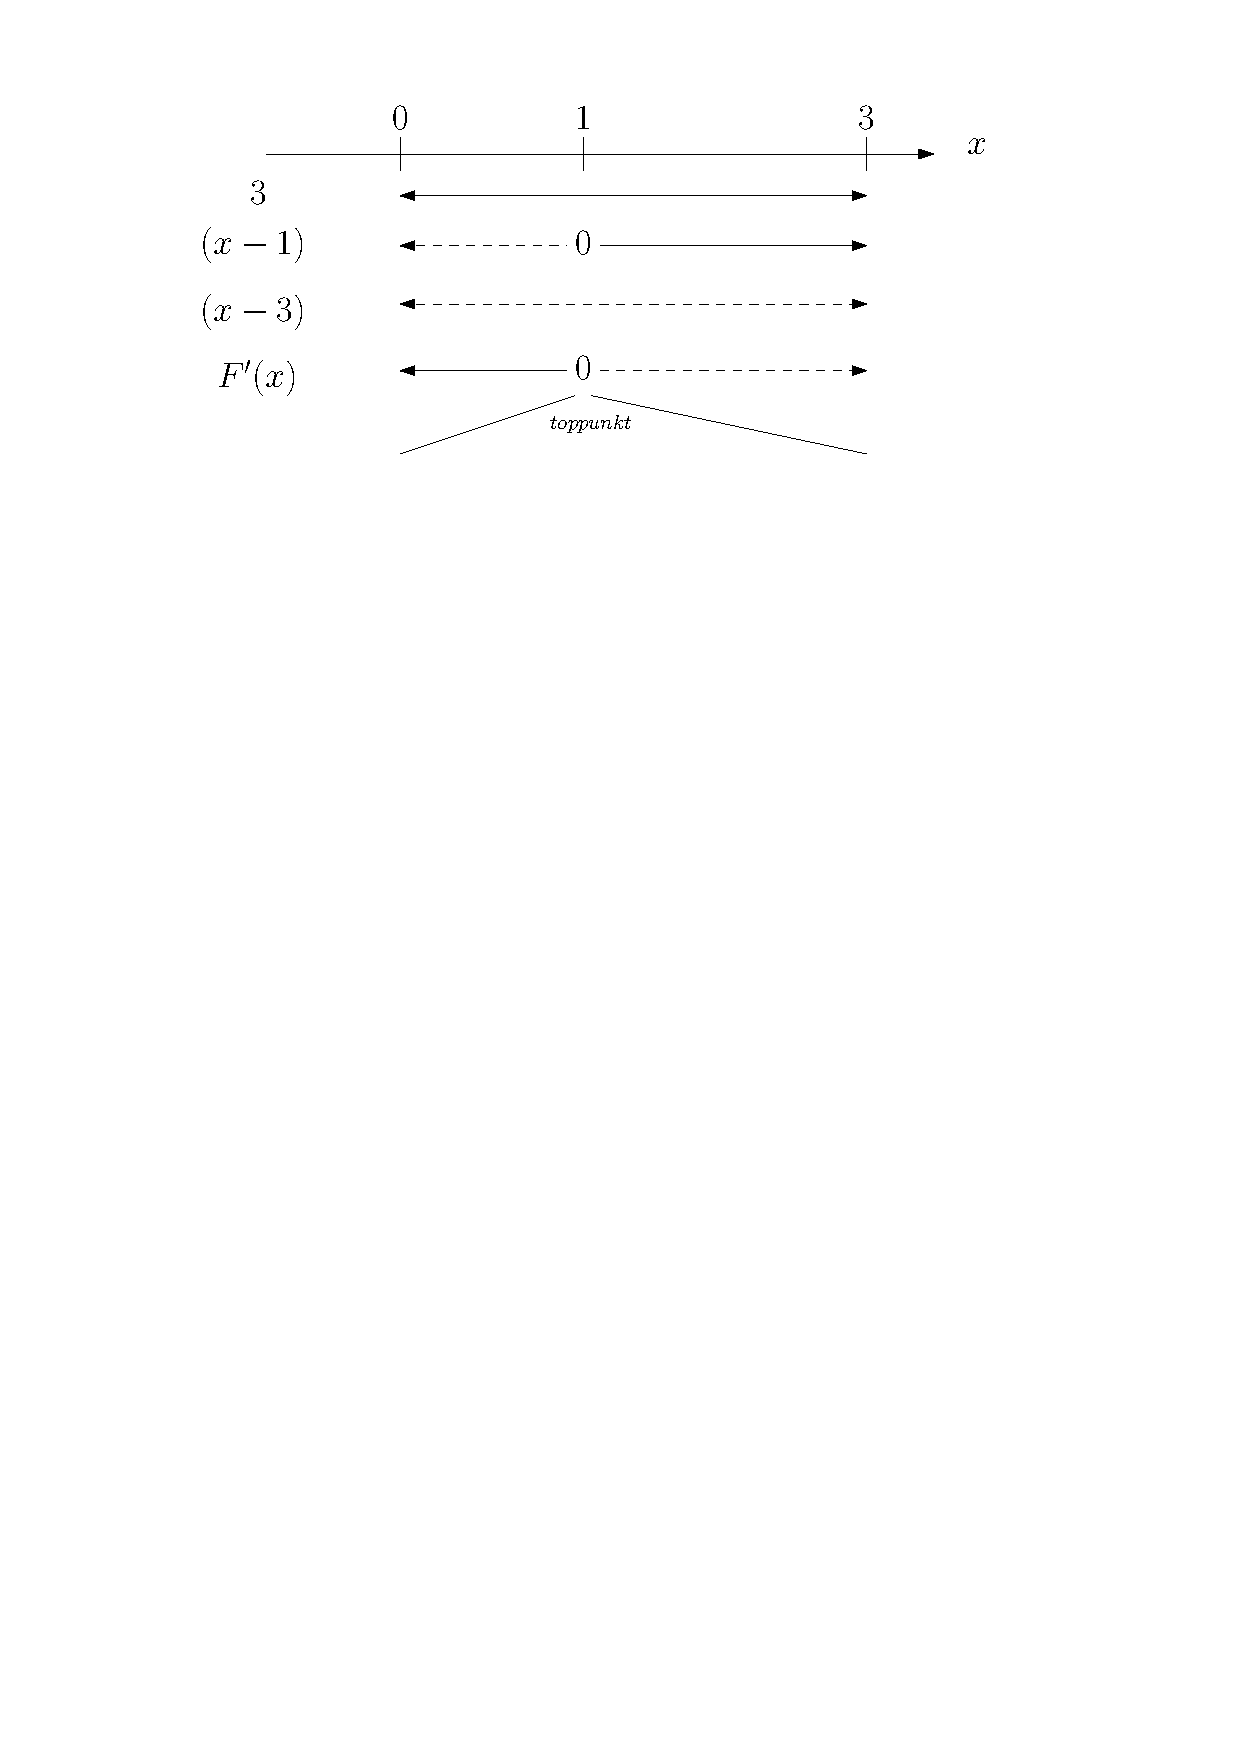
\includegraphics[width=0.725\linewidth]{figs/del1_oppg4b.pdf}
			\label{fig:del1_oppg4c}
		\end{figure}
		
		Ut i fra definisjonsmengden ser vi at det er kun $x = 1$ som gir mulighet for et toppunkt, og ut i fra fortegnslinjen ser vi at dette punktet faktisk er et toppunkt. Det vil si at \answer{arealet er størst når $x = 1$}.
		
	# Arealet finner vi ved å sette inn $x = 2$ i formelen for arealet.
	
	\[ F(2) = 2^3 - 6 \cdot 2^2 +9 \cdot 2 = 8 - 24 + 18 = 2 \]
	
	For å finne eventuelle andre x-verdier som gir dette arealet må vi sette opp likningen $x^3 - 6x^2 +9x = 2$. Vi vet fra over at x = 2 løser denne likningen, og det vil si at likningen $x^3 - 6x^2 +9x -2 = 0  $ (her har vi bare flyttet 2 over på venstre side) også har løsning $x=2$, som betyr at $(x-2)$ må være en faktor i polynomet på venstre side av likhetstegnet. Dette kan vi bruke til å gjøre en polynomdivisjon for å finne de eventuelle andre løsningene.
	
	\polylongdiv{x^3 - 6x^2 +9x -2}{x-2}
	
	Likningen over kan altså skrives som $(x^2 - 4x +1)(x-2) = 0$, og dette er oppfylt enten når $x = 2$ eller når $x^2 -4x +1 = 0$. Løsningene til den siste andregradslikningen kan vi finne ved hjelp av abc-formelen. Ved å bruke denne får vi at de to andre løsningene er $x = 2 \pm \sqrt{3}$. Siden $\sqrt{3} > 1$, vil løsningen $x = 2 + \sqrt{3}$ ligge utenfor definisjonsmengden. Derfor konkluderer vi med at \answer{det er en annen x-verdi som gir dette arealet, nemlig $x = 2 - \sqrt{3}$}.
	
\subsection*{Oppgave 5}
\begin{easylist}[enumerate]
	\ListProperties(Style2*=,Numbers=a,Numbers1=l,FinalMark={)})
	
	# Dette er et ordnet utvalg (rekkefølgen på tallene har betydning) med tilbakelegging (siden vi kan bruke tallene flere ganger). Vi skal velge mellom 10 tall 4 ganger. Antall mulige kombinasjoner er da gitt ved \answer{$10^4 = 10000$}.
	
	# Dette er et uordnet utvalg (siden tallene ikke trenger å være stilt inn i en bestemt rekkefølge) uten tilbakelegging (siden vi skal ha forskjellige tall). Vi skal gjøre 4 valg der antall valgmuligheter minsker med én for hvert valg. Antall kombinasjoner er da gitt ved
	
	$$\binom{10}{4} = \frac{10!}{4! \cdot (n-r)!} = \frac{10!}{4! \cdot 6!} = \frac{10 \cdot 9 \cdot 8 \cdot 7}{4 \cdot 3 \cdot 2 \cdot 1} = \frac{10}{2} \cdot \frac{9}{3} \cdot \frac{8}{4} \cdot 7 = 5 \cdot 3 \cdot 2 \cdot 7 = 210$$
	
	\answer{Det er altså 210 mulige kombinasjoner.}
	
	# TODO
	
	
	
	
\subsection*{Oppgave 6}
\begin{easylist}[enumerate]
	\ListProperties(Style2*=,Numbers=a,Numbers1=l,FinalMark={)})
	
	# Siden $M$ er midtpunktet på $AC$, betyr det at vi kan finne koordinatene til dette punktet slik:
	
	\[ \vec{OM} = \vec{OA} + \frac{1}{2} \vec{AC} = [3,-2] + \frac{1}{2} \cdot [-2,6]  = [2,1]\]
	
	\answer{Koordinatene til $M$ er (2,1) som vist over.}
	
	# For å lage en parameterframstilling for en rett linje trenger vi en retningsvektor til linja og et punkt på linja. Siden $l$ er midtnormalen til $AC$ betyr det at den må gå gjennom punktet $M$. Vi ser også at linja skjærer i punktet $(-1,0)$, og dermed kan vi finne en retningsvektor til linja ved å finne vektoren mellom dette punktet og $M$. 
	
	$[2-(-1),1-0] = [3,1]$.
	
	Deretter kan vi sette opp parameterframstillingen slik vi pleier
	
	\[
		l : \begin{cases}
				x = x_1 + at t\\
				y = y_1 + bt \\
		\end{cases}
	\]
	
	der $(x_1,y_1)$ er det faste punktet på linja og $[a,b]$ er retningsvektoren. Vi får da:
	
	
		\[
		l : \begin{cases}
		x = 2 + 3t t\\
		y = 1 + t \\
		\end{cases}
		\]
		
	# For å avgjøre om punktet ligger på linja, setter vi inn x- og y-verdien i parameterframstillingen og sjekker om vi får ut samme $t$-verdi.
	
	\begin{align*}
		12 & = 2 + 3t  && \frac{9}{2}  = 1 + t\\
		10 & = 3t  && \frac{9}{2} - 1  = t\\
		t & = \frac{10}{3} && t  = \frac{7}{2}
	\end{align*}
	
	Altså, \answer{punktet ligger ikke på linja.}
	
	# For å finne skjæringspunktet mellom to linjer kan vi bruke parameterframstillingene til de to linjene. Den ene har vi allerede, og parameterframstillingen for den andre kan vi finne på samme måte. Vi kaller midtnormalen til $AB$ for $m$ og midtpunktet på $AB$ for $M_1$. 

	$\vec{OM_1} = \vec{OA} + \frac{1}{2} \vec{AB} = [3,-2] + \frac{1}{2} \cdot [6,6] = [6,1]$
	
	Koordinatene til $M_1$ er $(6,1)$.  
	
	For å finne en retningsvektor for linja $m$ kan vi utnytte at midtnormalene står \textit{normalt} på den opprinnelige linja. Her skal vi vise to måter vi kan finne en slik retningsvektor.
	
	Første måte er å bruke at siden retningsvektoren til $AB$ er  $\vec{r} = [1,1]$, vil det si at stigningstallet til linja mellom $A$ og $B$ er 1. Stigningstaller for en linje som står normal på en annen linje med kjent stigningstall $a$ er $-\frac{1}{a}$, dermed vet vi at linja $m$ har stigningstall $-1$ og en retningsvektor for denne linja er da $[1,-1]$.
	
	Den andre måten vi kan finne dette på er å bruke at retningsvektoren til $AB$ og retningsvektoren til $m$ står vinkelrett på hverandre. Det betyr at skalarproduktet mellom dem er $0$. 
	
	\[ [1,1] \cdot [x,y] = 0 \]
	
	Dette blir null hvis x og y har samme tallverdi og motsatt fortegn. Mange løsninger er mulige, men for en retningsvektor betyr ikke valget av størrelsen på x og y så veldig mye, derfor velger vi for enkelthets skyld at de er $x = 1, y = -1$. 
	
	Parameterframstillingen for $m$ blir da
	
		\[
		m : \begin{cases}
		x = 6 + s\\
		y = 1 - s \\
		\end{cases}
		\]
		
		
		Skjæringspunktet mellom midtnormalene finner vi så ved å sette likningene for x og likningene for y lik hverandre i de to parameterframstillingene.
		
		
		\begin{align*}
		2 + 3t = 6 + s && 1 + t = 1 - s \\
		\end{align*}
		
		Fra likning 2 får vi $t = -s$, og dette setter vi så inn i likning 1 og får
		
		\begin{align*}
		2 + 3(-s) &= 6 + s \\
		2 - 3s & = 6 + s \\
		-4s & = 4 \\
		s = -1
		\end{align*}
		
		
		Setter vi dette inn i parameterframstillingen for $m$ finner vi skjæringspunktet.
		
		
			\[
			m : \begin{cases}
			x = 6 + s = 6 - 1 = 5\\
			y = 1 - s  = 1+1 = 2\\
			\end{cases}
			\]
	
		\answer{Skjæringspunktet mellom de to midtnormalene er (5,2)}
	
\subsection*{Oppgave 7}
\begin{easylist}[enumerate]
	\ListProperties(Style2*=,Numbers=a,Numbers1=l,FinalMark={)})

	
	
	
\end{easylist}	
\end{document}